%Methodology
\section{Methodology}

This study compares three recent methods for ensemble width estimation:
\begin{enumerate}
    \item a method based on an auditory model and decision trees (Section \ref{sec:methods:auditory}),
    \item a method using deep neural network (Section \ref{sec:methods:neural}),
    \item a method leveraging spatial spectrograms (Section \ref{sec:methods:spatial}).
\end{enumerate}
Initially, these methods were evaluated using anechoic recordings without noise. To test their performance in more ecological conditions, the methods were also tested using signals with predefined signal-to-noise ratios and simulated rooms with different reverberation characteristics (see Section \ref{sec:environmental}).

The objective of the methods incorporated in this study is to estimate the ensemble width ($\omega$) as illustrated in Figure \ref{fig:figx}. An ensemble is defined as a group of audio point sources positioned equidistantly around the listener on a circular virtual acoustic scene. The location of source $i$ is denoted by $\theta_i$. The~ensemble width ($\omega$) represents the angular distance between the two extreme point sources $(\max_i(\theta_i) - \min_i(\theta_i))$, while the ensemble location, represented by $\phi$, indicates the~midpoint angle between these extreme sources $((\max_i(\theta_i) + \min_i(\theta_i)) / 2)$. In this study, source locations are restricted to the frontal hemisphere, specifically $\theta \in [-45\degree, 45\degree]$ and $\omega \in [0\degree, 90\degree]$. It should be noted that although humans have some limited abilities to localize sound sources in the vertical plane, all sources in this study are positioned on the horizontal plane at ear level. These constraints reflect most real-world recording scenarios.


% % EQUATION 

% \begin{equation} \label{eq:1}
% \alpha + \beta = \gamma
% \end{equation}

% \subsection{Subsection Heading Here}
% Lorem ipsum dolor sit amet, consectetur adipiscing elit, sed do eiusmod tempor incididunt ut labore et dolore magna aliqua. Ut enim ad minim veniam, quis nostrud exercitation ullamco laboris nisi ut aliquip ex ea commodo consequat. Duis aute irure dolor in reprehenderit in voluptate velit esse cillum dolore eu fugiat nulla pariatur. Excepteur sint occaecat cupidatat non proident, sunt in culpa qui officia deserunt mollit anim id est laborum:

% \begin{itemize}
% 	\item one,
% 	\item two,
% 	\item three.
% \end{itemize}

% Lorem ipsum dolor sit amet, consectetur adipiscing elit, sed do eiusmod tempor incididunt ut labore et dolore magna aliqua. Ut enim ad minim veniam, quis nostrud exercitation ullamco laboris nisi ut aliquip ex ea commodo consequat. Duis aute irure dolor in reprehenderit in voluptate velit esse cillum dolore eu fugiat nulla pariatur. Excepteur sint occaecat cupidatat non proident, sunt in culpa qui officia deserunt mollit anim id est laborum. See Fig. \ref{fig:fig2}.

% \begin{figure}[htbp]
% 	\begin{center}
% 		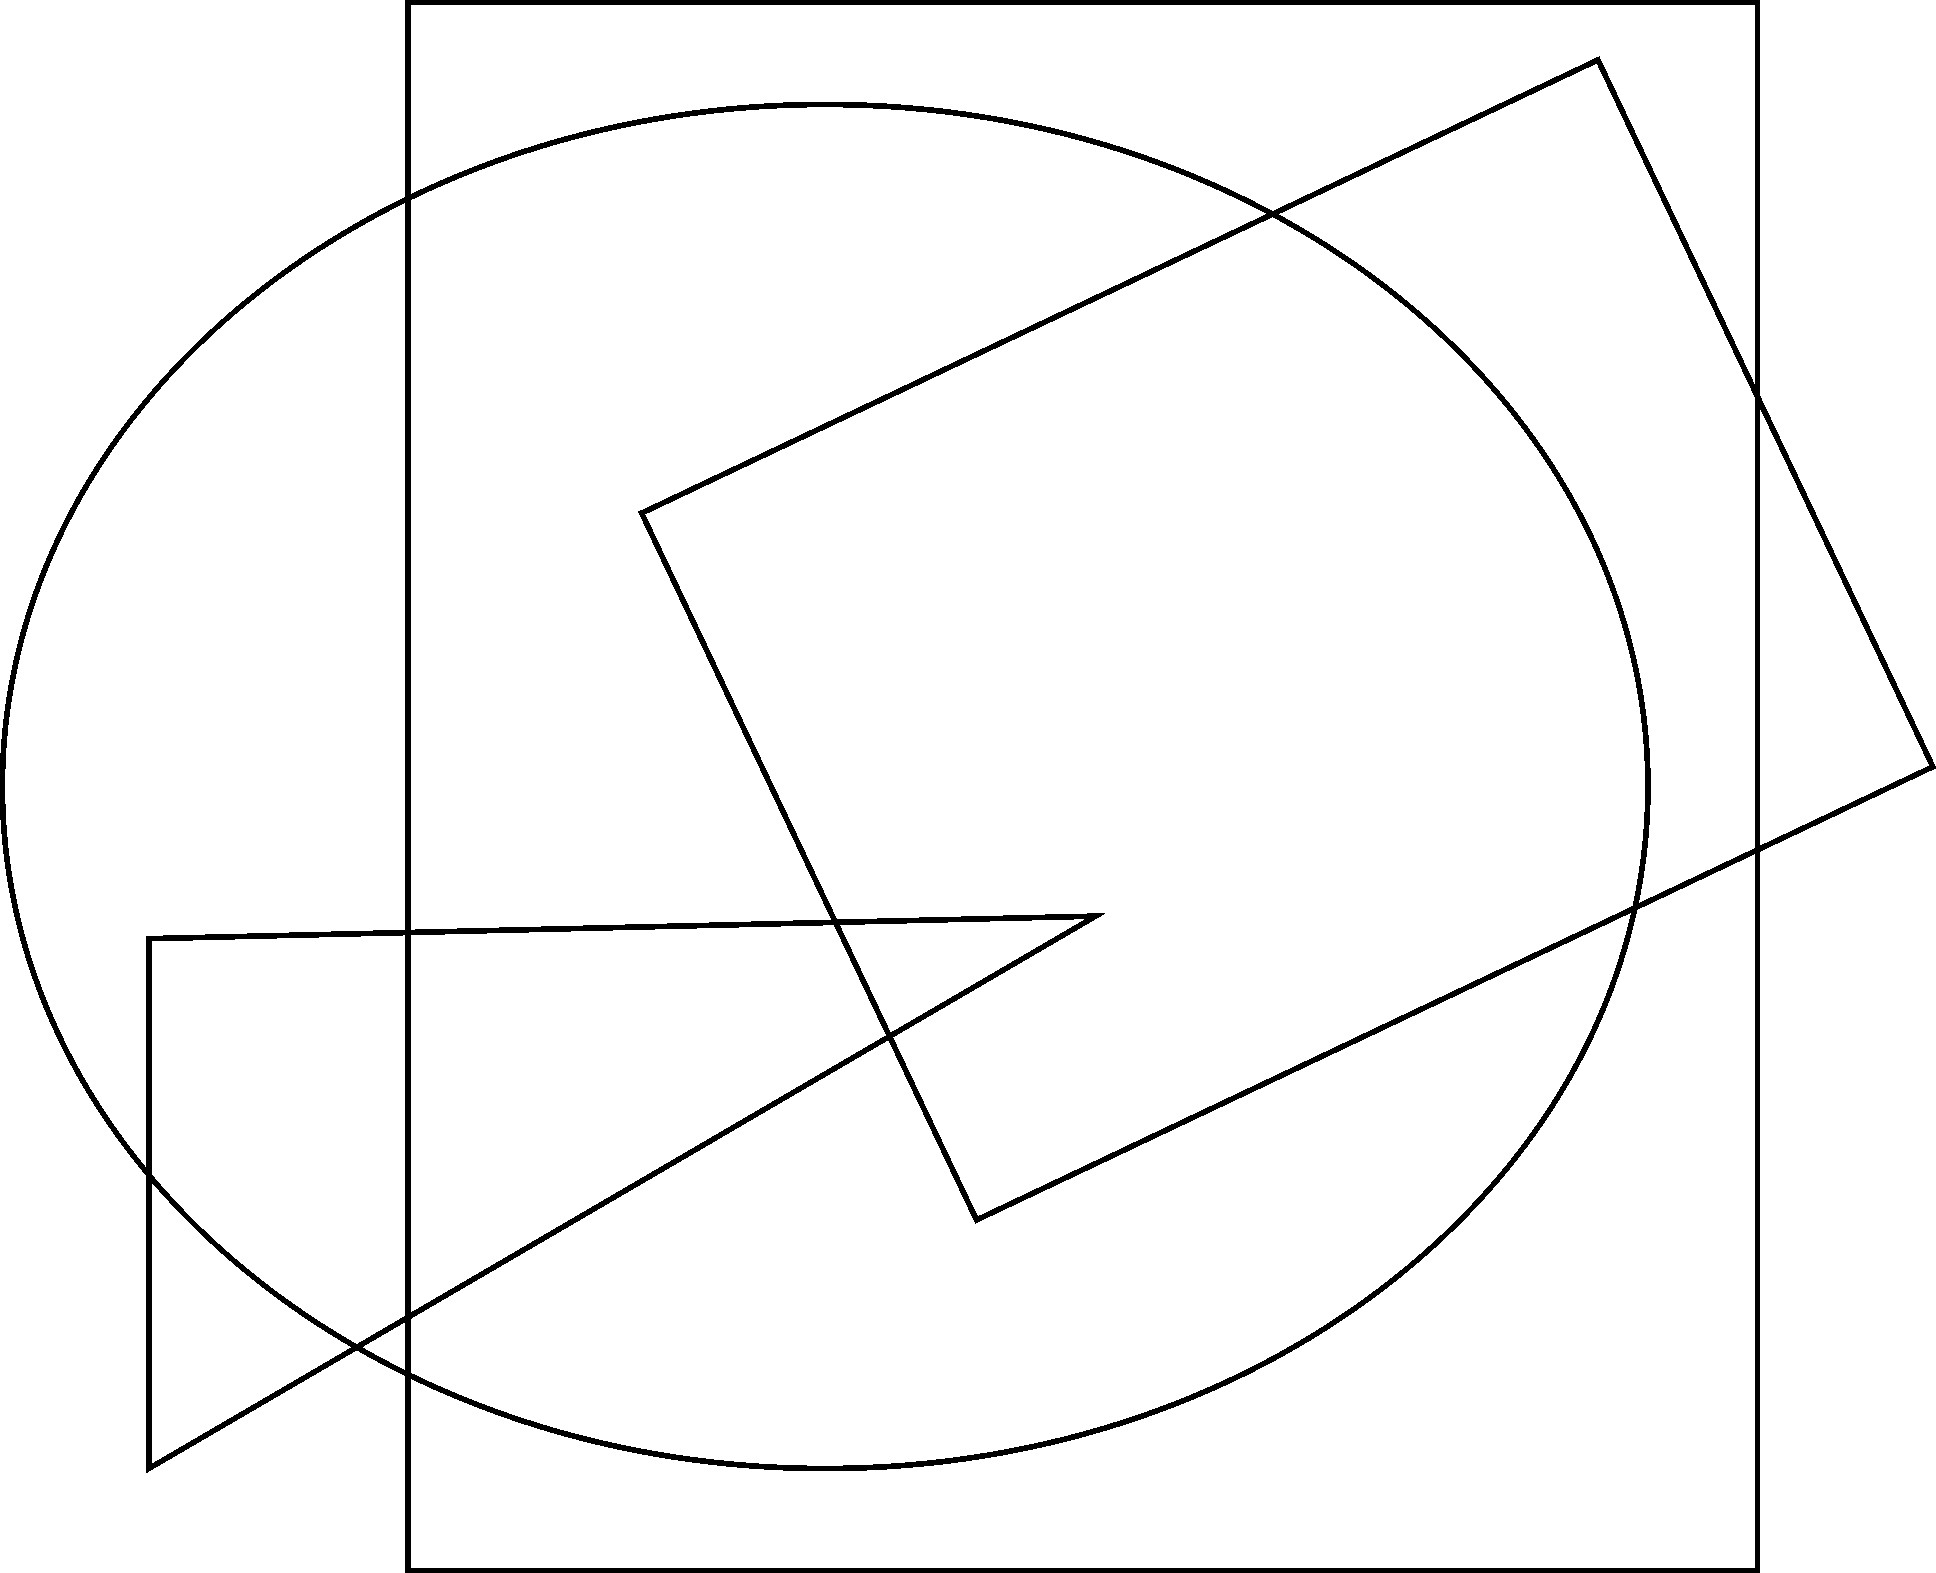
\includegraphics[width=0.8\linewidth]{img/fig2.jpg} 
% 	\end{center}
% 	\caption{Explain the significance of the figure in the caption} \label{fig:fig2}
% \end{figure}


%*****************************************

